%%%%%%%%%%%%%%%%%%%%%%%%%%%%%%%%%%%%%%%%%%%%%%%%%%%%%%%%%%%%%%%%%%%%%%%%%%%%%
%%%  Publishing and Consuming Government Linked Data on the Semantic Web  %%%
%%%%%%%%%%%%%%%%%%%%%%%%%%%%%%%%%%%%%%%%%%%%%%%%%%%%%%%%%%%%%%%%%%%%%%%%%%%%%

\documentclass[a4paper,11pt]{report}
%\usepackage[latin1]{inputenc}
\usepackage[english]{babel}
\usepackage{graphicx} 
\usepackage{pdfpages}
\usepackage{fancyvrb}
\usepackage{pdflscape}
\usepackage{fancyhdr}
\usepackage[utf8]{inputenc}
\usepackage{amssymb}
\pagestyle{fancy}
\setcounter{tocdepth}{3}
\usepackage{tabularx}
\usepackage{url}

\bibliographystyle{unsrt}

%\fancyhead[CO,CE]{---MidTerm Report--}
\fancyhead[RO, LE] {\thepage}
\renewcommand{\headrulewidth}{0.4pt}
\renewcommand{\footrulewidth}{0.4pt}

%%%%%%%%%%%%%%%%%%%%%%%%%%%%%%%
%%%  Beginning of document  %%%
%%%%%%%%%%%%%%%%%%%%%%%%%%%%%%%

\begin{document}

\begin{titlepage}
\begin{center}

\includegraphics[width=5cm]{EURECOM_logo_quadri}
\\[3cm]
\textbf{\Huge{MidTerm Report}}
\\[4cm]
\textbf{\textsc{\LARGE{Publishing and Consuming Government Linked Data on the Semantic Web}}}
\\[0.5cm]
\LARGE{Ghislain Auguste Atemezing}
\\[0.5cm]
\small{EURECOM-Multimedia Communications}
\\
\large{Institut Mines-T\'{e}l\'{e}com}
\\
\large{December 19th, 2012}
\\[5cm]
\columnsep3cm
\begin{tabular}{p{8cm} p{8.5cm}}
\small{\textbf{Supervisor:}\newline
Rapha\"el Troncy} 
&
\small{\textbf{EURECOM\newline Multimedia Department}}
\end{tabular}
\end{center}
\end{titlepage}

 \tableofcontents

%%%%%%%%%%%%%%%%%%%
%%%   Abstract  %%%
%%%%%%%%%%%%%%%%%%%

\chapter*{Abstract}
\addcontentsline{toc}{chapter}{Abstract}

The need for geolocation is crucial for many applications for both human and software agents. More and more data is opened and interlinked using Linked Data principles, and it is worth modeling geographic data efficiently by reusing as much as possible from existing ontologies or vocabularies that describe both the geospatial features and their shapes. Our aim is to contribute to the actual efforts in representing geographic objects with attributes such as location, points of interest (POI), and addresses in the web of data, with a special focus on the French territory.
As we publish data in RDF graphs, we are also aware of making them useful for the users. For that, we not only develop innovative applications to show up the value of data visualizations, but rather go beyond it. The challenge is to detect patterns to automatically develop an application using adequate visualization widgets in an affordable effort.  

%%%%%%%%%%%%%%%%%%%%%%%%%%%%%%%%%
%%%  Chapter:Reseach Problems %%%
%%%%%%%%%%%%%%%%%%%%%%%%%%%%%%%%%


\chapter{Research Problems}

\section{Introduction}
The Web is currently in a transition phase. After having been accessible on personal computers, it is now 
quickly moving to more and more ubiquity and entering in every part and moment of our lives. New 
devices and new ways to use them are being created. The ubiquity of the Web also creates an unseen 
abundance of information. Data is flowing onto the Web, created by users, generated by sensors, and 
stored in ever growing data farms. Geographic data is widely present on the web as they are used for location 
of Point of Interest. At the same time, many organizations are moving from legacy data stored in their databases
to structured data on the web. Structured data is already present in the many databases, metadata attached to medias, and in the millions of spreadsheets created everyday across the world. 

However, the recent emergence of linked data radically changes the way structured data is being considered. By giving standard formats for the publication and interconnection of structured data, linked data transforms the Web into a giant database. While making data available on the web, we need to build meaningful applications to show the value of all the huge data so that users could easily explore it, and derive new insights for it. As many information visualization tools are already present in InfoVis community\footnote{http://en.wikipedia.org/wiki/Information\_visualization}, their easy adoption and usage for displaying structured data raise new challenges. Those challenges are twofolds:
\begin{itemize}
\item How to characterize semantic web applications in terms of tools, widgets that can easily visualize RDF datasets.
\item Mining heterogeneous structured data to derive patterns for automatically recommend the adequate visualization tool to help users building innovative applications in an affordable time.
\end{itemize}

%%%%%%%%%%%%%%%%%%%%%%%%%%%%%%
%%% section contributions %%%%
%%%%%%%%%%%%%%%%%%%%%%%%%%%%%%

\section{Contributions}
   %TODO: Extend this section with the outline of my work in those two directions: geoData and visualization
The present report aims at giving a summary of the activities we have been accomplishing
during the first year of our thesis entitled: \textbf{``Publishing and Consuming Government Linked Data on the Semantic Web''}. Our main purpose was to first understand the problematic by an extensive state-of-the-art in : 
\begin{itemize}
\item (i)- Geographic Information on the Web of data, and 
\item (ii) visualization tools for building innovative applications consuming structured data. 
\end{itemize}

%%%%%%%%%%%%%%%%%%%%%%%%%%%%%%%%%%%%%%%%%%%%%%%%%%%%%%%%
%%%  Chapter:Modeling Geographic Information in LOD  %%%
%%%%%%%%%%%%%%%%%%%%%%%%%%%%%%%%%%%%%%%%%%%%%%%%%%%%%%%%

\chapter{Modeling Geographic Information in LOD}

\section{Introduction}
The need for geolocation is crucial for many applications for both human and software agents. More and more data is opened and interlinked using Linked Data principles, and it is worth modeling geographic data efficiently by reusing as much as possible from existing ontologies or vocabularies that describe both the geospatial features and their shapes. In the first part of our work, we survey different modeling approaches used by the Geographic Information System (GIS) and the Linked Open Data (LOD) communities. Our aim is to contribute to the actual efforts in representing geographic objects with attributes such as location, points of interest (POI), and addresses on the web of data. We focus on the French territory and we provide examples of representative vocabularies that can be used for describing geographic objects. We propose some alignments between various vocabularies (DBpedia, GeoNames, Schema.org, LinkedGeoData, Foursquare, etc.) in order to enable interoperability while interconnecting French geodata with other datasets. In France, there is  currently a joint effort to publish geographic information in RDF  and interlink them with relevant datasets. GeOnto is an ontology describing geospatial features for the French territory. We have proposed to align GeOnto with other popular vocabularies in the geospatial domain, using Silk for schema mapping and we have evaluated the results. We studied how to extend the model to take into account efficient modeling for complex geometries. By doing so, tackle the complex geometry representation issues in the Web of Data, describing the state of implementations of geo-spatial functions in triple stores and comparing them to the new GeoSPARQL standard.  We finally made some recommendations and advocate for the reuse of the NeoGeo ontology within GeOnto to better address the IGN requirements.
This work has lead to two publications [2,4]

\section{Geographic information in the Web of Data}                         \label{sec:geo-in-web-of-data}

\subsection{LOD Cloud Review}
The recent publication of statistics concerning the actual usage of vocabularies on the LOD cloud\footnote{\url{http://stats.lod2.eu}} provides not only an overview of best practice usage recommended by Tim Berners-Lee\footnote{\url{http://www.w3.org/DesignIssues/LinkedData.html}}, but also provides a rapid view of the vocabularies re-used in various datasets and domains. Concerning the geographic domain, the results show that W3C Geo\footnote{\url{http://www.w3.org/2003/01/geo/wgs84_pos}} is the most widely used vocabulary, followed by the \texttt{spatialrelations}\footnote{\url{http://data.ordnancesurvey.co.uk/ontology/spatialrelations}} ontology of Ordnance Survey (OS). At the same time, the analysis reveals that the property \texttt{geo:geometry} is used in $1,322,302,221$ triples, exceeded only by the properties \texttt{rdf:type} ($6,251,467,091$ triples) and \texttt{rdfs:label}($1,586,115,316$ triples). This shows the importance of geodata on the web. Table~\ref{tab:vocabLOD} summarizes the results for four vocabularies (WGS84, OS spatial relation, Geonames ontology and OS admin geography) where the number of datasets using these vocabularies and the actual number of triples are computed.
\begin{table*}[!htbp]
\centering{
\begin{tabular}{|l|r|r|c| }
\hline
\multicolumn{1}{|c|} {Ontologies} & \multicolumn{1}{c|}{\#Datasets using} & \multicolumn{1}{c|}{\#Triples}& \multicolumn{1}{c|}{SPARQL endpoint}\\
\hline
W3C Geo  &   21 & 15 543 105 & LOD cache\\
OS spatialrelations &   10 & 9 412 167 & OS dataset\\
Geonames ontology &   5 & 8 272 905 & LOD cache\\
UK administrative-geography &   3 &  229 689 & OS dataset \\
\hline
\end{tabular}
\caption{Statistics on the usage of the four main geographic vocabularies (LOD cache should be understood as \texttt{http://lod.openlinksw.com/sparql/}). There are many more vocabularies used in the LOD cloud that contain also geographical information but that are never re-used.}
\label{tab:vocabLOD}
}
\end{table*}


\subsection{Geodata Provider and Access}
So far, the Web of data has taken advantage of geocoding technologies for publishing large amounts of data. For example, Geonames provides more than 10 millions records (e.g. $5,240,032$ resources of the form \url{http://sws.geonames.org/10000/}) while LinkedGeoData has more than $60,356,364$ triples. All the above mentioned data are diverse in their structure, the access point (SPARQL endpoint, web service or API), the entities they represent and the vocabularies used for describing them. Table~\ref{tab:srce-data} summarizes for different providers the number of geodata available (resources, triples) and how the data can be accessed.
\begin{table}[!htbp]
\centering{
\begin{tabular}{|ll|r|r|}
\hline
\multicolumn{2}{|c}{\textbf{Provider}} & \multicolumn{1}{|c}{\textbf{\#Geodata}} & \multicolumn{1}{|c|}{\textbf{Data access}}\\
\hline
\multicolumn{2}{|l|}{DBpedia} & 727 232 triples & SPARQL endpoint\\
\multicolumn{2}{|l|}{Geonames} & 5 240 032 (feature). &  API \\
\multicolumn{2}{|l|}{LinkedGeoData} & 60 356 364 triples & SPARQL endpoint, Snorql\\
\multicolumn{2}{|l|}{Foursquare} & n/a & API\\
\multicolumn{2}{|l|}{Freebase} & 8,5MB  & RDF Freebase Service\\
\multicolumn{2}{|l|}{Ordnance Survey(Cities)} & 6 295 triples  & Talis API \\
\multicolumn{2}{|l|}{GeoLinkedData.es} & 101 018 triples  & SPARQL endpoint \\
\multicolumn{2}{|l|}{Google Places} & n/a  & Google API \\
\multicolumn{2}{|l|}{GADM project data} & 682 605 triples & Web Service \\
\multicolumn{2}{|l|}{NUTS project data} & 316 238 triples & Web Service \\
\multicolumn{2}{|l|}{IGN experimental} & 629 716 triples & SPARQL endpoint \\
\hline
\end{tabular}
\caption{Geodata by provider and their different access type}
\label{tab:srce-data}
}
\end{table}


\section{Geodata Modeling Approach}                                         \label{sec:modeling-approach}

\subsection{Vocabularies for Features}
Modeling of features can be grouped into four categories depending on the structure of the data, the intended purpose of the data modeling, and the (re)-use of other resources.
\begin{itemize}
  \item (i): One way for structuring the features is to define high level codes (generally using a small finite set of codes) corresponding to specific
      types. Further, sub-types are attached to those codes in the classification. This approach is used in the Geonames ontology\footnote{\url{http://geonames.org/ontology/ontology_v3.0.rdf}} for codes and classes (A, H, L, P, R, S, T, U, V), with each of the letter corresponding to a precise category (e.g: A for administrative borders). Classes are then defined as \texttt{gn:featureClass a skos:ConceptScheme}, while codes are \texttt{gn:featureCode a skos:Concept}.
  \item (ii): A second approach consists in defining a complete standalone ontology that does not reuse other vocabularies. A top level class is used under which a taxonomy is formed using the \texttt{rdfs:subClassOf} property. The LinkedGeoData ontology\footnote{\url{http://linkedgeodata.org/ontology}} follows this approach, where the $1294$ classes are built around a nucleus of $16$ high-level concepts which are: \texttt{Aerialway, Aeroway, Amenity, Barrier, Boundary, Highway, Historic, Landuse, Leisure, ManMade, Natural, Place, Power, Route, Tourism} and \texttt{Waterway}. The same approach is used for the French GeOnto ontology (Section~\ref{sec:alignment}), which defined two high-level classes \texttt{ArtificialTopographyEntity} and \texttt{Natural\-TopographyEntity} with a total of $783$ classes.
  \item (iii): A third approach consists in defining several smaller ontologies, one for each sub-domain. An ontology network is built with a central ontology used to interconnect the different other ontologies. One obvious advantage of this approach is the modularity of the conceptualizing which should ease as much as possible the reuse of modular ontologies. Ordnance Survey (OS) follows this approach providing ontologies for administrative regions\footnote{\url{http://www.ordnancesurvey.co.uk/ontology/admingeo.owl}}, for statistics decomposition\footnote{\url{http://statistics.data.gov.uk/def/administrative-geography}} and for postal codes\footnote{\url{http://www.ordnancesurvey.co.uk/ontology/postcode.owl}}. The \texttt{owl:imports} statements are used in the core ontology. Similarly, GeoLinkedData makes use of three different ontologies covering different domains.
  \item (iv): A fourth approach consists in providing a \textit{nearly flat list} of features or points of interest. This is the approach followed by popular Web APIs such as Foursquare types of venue\footnote{\url{http://aboutfoursquare.com/foursquare-categories/}} or Google Place categories\footnote{\url{https://developers.google.com/maps/documentation/places/supported_types}}. For this last approach, we have built an associated OWL vocabulary composed of alignments with other vocabularies.
\end{itemize}

\subsection{Vocabularies for Geometry Shape}
The geometry of a point of interest is also modeled in different ways. We complete here the survey started by Salas and Harth~\cite{Salas2011}:
\begin{itemize}
  \item \textit{Point representation}: the classical way to represent a location by providing the latitude and longitude in a given coordinate reference system (the most used on the web is the WGS84 datum represented in RDF by the W3C Geo vocabulary). For example, Geonames defines the class \texttt{gn:Feature a skos:ConceptScheme} as a \texttt{SpatialThing} in the W3C Geo vocabulary.
  \item \textit{Rectangle} (``bounding box''): which represents a location with two points or four segments making a geo-referenced rectangle. In this way of modeling, the vocabulary provides more properties for each segment. The FAO Geopolitical ontology\footnote{\url{http://www.fao.org/countryprofiles/geoinfo/geopolitical/resource/}} uses this approach.
  \item \textit{List of Points}: the geometry shape is a region represented by a collection of points, each of them being described by a unique RDF node identified by a lat/lon value. The \texttt{Node} class is used to connect one point of interest with its geometry representation. The POI are modeled either as \texttt{Node} or as \texttt{Waynode} (surfaces). This approach is followed by LinkedGeoData~\cite{linkedgeodata}.
  \item \textit{Sequence of Points}: the geometry shape is represented by a group of RDF resources called a ``curve'' (similar to LineString of GML). The POI is connected to its geometry by the property \texttt{formedBy} and an attribute \texttt{order} to specify the position of each node in the sequence. This approach is the one used in GeoLinkedData~\cite{deLeon2010}.
  \item \textit{Literals}: the vocabulary uses a predicate to include the GML representation of the geometry object, which is embedded in RDF as a literal. This approach is followed by Ordance Survey~\cite{Goodwin2008}.
  \item \textit{Structured representation}: the geometry shape is represented as a typed resource. In particular, polygons and lines are represented with an RDF collection of basic W3C Geo points. This approach is used by the NeoGeo vocabulary\footnote{\url{http://geovocab.org/doc/neogeo/}}.
\end{itemize}

%%%%%%%%%%%%%%%%%%%%%%%%%%%%%%%%%%%%%%%%%%%%%%%%%%%%%%%%
%%%  4. Scenario: 7\inst{th} Arrondissement of Paris %%%
%%%%%%%%%%%%%%%%%%%%%%%%%%%%%%%%%%%%%%%%%%%%%%%%%%%%%%%%

\section{Scenario: 7th Arrondissement of Paris}                      \label{sec:scenario}
The 7th arrondissement of Paris is one of the 20 arrondissements (administrative districts) of the capital city of France. It includes some of Paris's major tourist attractions such as the Eiffel Tower, some world famous museums (e.g: \textit{musée d'Orsay}) and contains a number of French national institutions, including numerous government ministries\footnote{\url{http://en.wikipedia.org/wiki/7th_arrondissement_of_Paris}}. We use it throughout this paper to highlight the diversity of representations one can use for this geographical entity. We assume that this district should be modeled as a POLYGON composed of a number of POINTs needed to ``interpolate'' its effective boundaries. We assume the use of the WGS84\footnote{\url{http://en.wikipedia.org/wiki/World_Geodetic_System}} geodetic system.

\subsection{DBpedia Modeling}
We provide below an excerpt of the DBpedia description for this resource.
{\scriptsize
\begin{verbatim}
  dbpedia:7th_arrondissement_of_Paris a gml:_Feature ;
    a <http://dbpedia.org/class/yago/1900SummerOlympicVenuEs>
    rdfs:label "7. arrondissementti (Pariisi)"@fi; (14 different languages)
    dbpprop:commune "Paris" ;
    dbpprop:département  dbpedia:Paris ;
    dbpprop:région dbpedia:Île-de-France_(region) ;
    grs:point "48.85916666666667 2.312777777777778" ;
    geo:geometry "POINT(2.31278 48.8592)" ;
    geo:lat "48.859165"^^xsd:float;
    geo:long "2.312778"^^xsd:float.
\end{verbatim}
}
First, we observe that the type \texttt{gml:\_Feature} and the property \texttt{grs:point} are not resolvable since there are no OWL ontologies that provide a description of them. Second, the property \texttt{geo:geometry} used by DBpedia is not defined in the WGS84 vocabulary. For the geometry, the 7th arrondissement is a simple POINT defined by a latitude and a longitude.

\subsection{Geonames Modeling}
In Geonames, the 7th arrondissement is considered as a 3rd order administrative division, represented by a POINT for the geometry model. The RDF description of this resource gives other information such as the alternate name in French, the country code and the number of inhabitants.
{\scriptsize
\begin{verbatim}
  gnr:6618613 a gn:Feature ;
    gn:name "Paris 07";
    gn:alternateName "7ème arrondissement";
    gn:featureClass gn:A [
      a skos:ConceptScheme ;
      rdfs:comment "country, state, region ..."@en .
    ] ;
    gn:featureCode gn:A.ADM4 [
      a skos:Concept ;
      rdfs:comment "a subdivision of a third-order administrative division"@en .
    ];
    gn:countryCode "FR";
    gn:population "57410";
    geo:lat "48.8565";
    geo:long "2.321".
\end{verbatim}
}

\subsection{LinkedGeoData Modeling}
In LinkedGeoData, the district is a \texttt{lgdo:Suburb rdfs:subClassOf ldgo:Place}. Its geometry is still modeled as a POINT and not as a complex geometry of type POLYGON as we could have expected for this type of spatial object.
{\scriptsize
\begin{verbatim}
  lgd:node248177663 a lgdo:Suburb ;
    rdfs:label "7th Arrondissement"@en , "7e Arrondissement" ;
    lgdo:contributor lgd:user13442 ;
    lgdo:ref%3AINSEE 75107 ;
    lgdp:alt_name "VIIe Arrondissement" ;
    georss:point "48.8570281 2.3201953" ;
    geo:lat 48.8570281 ;
    geo:long 2.3201953 .
\end{verbatim}
}

\subsection{Discussion}
These samples from DBpedia, Geonames and LinkedGeoData give an overview of the different views of the same reality, in this case the district of the 7th Arrondissement in Paris. Regarding the ``symbolic representation'', two datasets opted for ``Feature'' (DBpedia and Geonames) while LGD classifies it as a ``Suburb'' or ``Place''. They all represent the shape of the district as a POINT which is not very efficient if we consider a query such as \emph{show all monuments located within the 7th arrondissement of international importance}. To address this type of query and more complicated ones, there is a need for more advanced modeling as we describe in the next section.


%%%%%%%%%%%%%%%%%%%%%%%%%%%%%%%%%%%%%
%%%  5. Aligning Geo Vocabularies %%%
%%%%%%%%%%%%%%%%%%%%%%%%%%%%%%%%%%%%%

\section{Aligning Geo Vocabularies}                                         \label{sec:alignment}
IGN is a public service in France in charge of describing, from the physical and geometry point of view, the surface of the French territory and the occupation of the land, and to elaborate and update continuously the forestal resources. They are also experimenting in exposing some of their data as Linked Data and act as an important provider in the \url{http://data.gouv.fr} portal.

\subsection{Existing Vocabularies}
IGN has developed two complementary vocabularies (GeOnto and bdtopo) which differ in their provenance but have the same scope, which is to describe geographic entities in the French territory. GeOnto is the product of a research project\footnote{\url{http://geonto.lri.fr/Livrables.html}} aiming at building and aligning heterogeneous ontologies in the geographic domain. The ``light'' version of the final ontology\footnote{\url{http://semantics.eurecom.fr/datalift/tc2012/vocabs/GeoOnto/}} defines two top classes for a total of $783$ classes and $17$ properties ($12$ DP / $5$ OP). GeOnto has labels in both French and English, but has no comments specified for the resources. The bdtopo ontology is derived from a geospatial database with the same name. It contains $237$ classes and $51$ properties ($47$ DP / $4$ OP). All the labels and comments are in French.

\subsection{GeOnto Alignment Process}
The first step towards interoperability of French geographic features and the existing vocabularies is to align GeOnto to other vocabularies. We choose GeOnto because it covers a large number of categories and also has labels in English. We have performed the alignment with five OWL vocabularies (bdtopo, LGD, DBpedia, Schema.org and Geonames) and two flat taxonomies (Foursquare, Google Place). For the latter, we have transformed the flat list of types and categories into an OWL ontology. For each alignment performed, we only consider \texttt{owl:equivalentClass} axioms. We use the Silk tool \cite{Julius09} to compute the alignment using two metrics for string comparison: the \textit{levenshteinDistance} and \textit{jaro} distances. They work on the English labels except for the alignment with bdtopo where we use the French labels. We apply the average aggregation function on these metrics with an empirically derived threshold. However, for generating the final mapping file for vocabularies of small size, we manually validate and insert relations of type \texttt{rdfs:subClassOf}. The threshold to validate the results is set to $100$\% for links considered to be correct and greater than $40$\% for links to be verified. The alignment with Geonames is special, considering the property restriction used in the ontology for codes.

Table~\ref{tab:mappings} summarizes the result of the alignment process between GeOnto and the existing vocabularies/taxonomies. All the resources of this work are available at \url{http://semantics.eurecom.fr/datalift/tc2012/}.
\begin{table}
\centering{
\begin{tabularx}{\textwidth}{|X|X|r|}%{|l|l|c|}
\hline
\textbf{Vocabulary}    	& \textbf{\#Classes} 	& \textbf{\#Aligned Classes}    \\ \hline
LGD 			& \texttt{owl:Class}:$1294$     &  $178$			            \\  \hline

DBpedia     	& \texttt{owl:Class}:$366$ 	    & $42$			   				 \\ \hline
				
Schema.org 		& \texttt{owl:Class}:$296$ 	    &  $52$			     			 \\ \hline
				
Geonames		& \texttt{skos:ConceptScheme}:$12$  &  --			    	 	  \\
               	& \texttt{skos:Concept}:$699$       &  $287$               			\\ \hline
Foursquare 		& $359$ 	    			        & $46$ 			 			   \\ \hline
Google Place 	& $126$ 	  			            & $41$ 			 	 			\\ \hline
bdtopo 			& \texttt{owl:Class}:$237$ 	  	    & $153$ 			 	 		\\ \hline
\end{tabularx}
\caption{Results of the alignment process between GeOnto and existing vocabularies/taxonomies.}
\label{tab:mappings}
}
\end{table}

In general, we obtain good results with Silk, with precision beyond $80$\%: Google Place: $94$\%, LGD: $98$\%, DBpedia: $89$\%, Foursquare: $92$\% , Geonames: $87$\% and bdtopo: $92$\%. We obtained a precision of only $50$\% with schema.org due to numerous fine-grained categories that are badly aligned (e.g. \texttt{ign:Berge owl:equivalentClass schema:Park}).

%%%%%%%%%%%%%%%%%%%%%%
%%%  6. Challenges %%%
%%%%%%%%%%%%%%%%%%%%%%

\section{Challenges}                                                        \label{sec:challenges}

\subsection{GeoSPARQL}
OGC has adopted the GeoSPARQL standard to support both representing and querying geospatial data on the Semantic Web. The standard document~\cite{ogc2012} contains 30 requirements. It also defines a vocabulary for representing geospatial data in RDF and provides an extension to the SPARQL query language for processing geospatial data. The proposed standard follows a modular design with five components: (i) A \textit{core component} defining top-level RDFS/OWL classes for spatial objects; (ii) a \textit{geometry component} defining RDFS data types for serializing geometry data, RDFS/OWL classes for geometry object types, geometry-related RDF properties, and non-topological spatial query functions for geometry objects; (iii) a \textit{geometry topology component} defining topological query functions; (iv) a \textit{topological vocabulary component} defining RDF properties for asserting topological relations between spatial objects; and (iv) a \textit{query rewrite component} defining rules for transforming a simple triple pattern that tests a topological relation between two features into an equivalent query involving concrete geometries and topological query functions. Each of the components described above has associated requirements. Concerning the vocabulary requirements, the document specifies seventeen requirements presented in the GeoSPARQL draft document.


Based on the GeoSPARQL requirements, we were interested in comparing some geospatial vocabularies\footnote{\url{http://labs.mondeca.com/dataset/lov/vocabularySpace_Space.html}} to see how far they take already into account topological functions and which are the standard they followed among OpenGIS Simple Features (SF), Region Connection Calculus (RCC) and Egenhofer relations. We find that the NeoGeo (Spatial and Geometry) and OS Spatial vocabularies have integrated in their modeling partial or full aspects of topological functions as summarized in Table~\ref{tab:geosparql}.

As geodata has to be stored in triple stores with efficient geospatial indexing and querying capabilities, we also survey the current state of the art  in supporting simple or complex geometries and topological functions compatible with SPARQL 1.1. Table~\ref{tab:triplestore} shows which triple stores can support part of the GeoSPARQL standard regarding serialization and spatial functions.


\subsection{Some Recommendations}
The alignment of GeOnto provided in the previous section enables interoperability of symbolic descriptions. The need for a better choice of geometric structure, typically the choice between literal versus structured representations depends on three criteria: (i) the coverage of all the complex geometries as they appear in the data; (ii) a rapid mechanism for connecting ``features'' to their respective ``geometry''; (iii) the possibility to serialize geodata into traditional formats used in GIS applications (GML, KML, etc.) and (iv) the choice of triple stores supporting as many as possible functions to perform quantitative reasoning on geodata. It is clear that a trade-off should be taken depending on the technological infrastructure (e.g: data storage capacity, further reasoning on specific points on a complex geometry).
\begin{itemize}
\item\textbf{Complex Geometry Coverage:} We have seen that on the Web of Data, there are few modeling of geodata with their correct shape represented as a LINE or POLYGON. However, some content providers (e.g. IGN) need to publish all types of geodata including complex geometries representing roads, rivers, administrative regions, etc. Two representations are suitable: \textit{OS Spatial} and \textit{NeoGeo} ontologies (Table~\ref{tab:reqgeosparql}). Direct representation of the GeoSPARQL vocabulary is also suitable.
\item \textbf{Features connected to Geometry:} In modeling geodata, we advocate a clear separation between the features and their geometry. This is consistent with the consensus obtained from the different GeoVocamps\footnote{\url{http://www.vocamp.org}} and the outcome of this approach is expressed in the modeling design of NeoGeo. The top level classes \texttt{spatial:Feature} and \texttt{geom:Geometry}are connected with the property \texttt{geom:geometry}.
\item \textbf{Serialization and Triple stores:} We also advocate the use of properties that can provide compatibility with other formats (GML, KML, etc.). This choice can be triple store independent, as there could be ways to use content-negotiation to reach the same result. In Table \ref{tab:triplestore}, \texttt{Open Sahara}\footnote{\url{http://www.opensahara.com}}, \texttt{Parliament }\footnote{\url{http://geosparql.bbn.com}},  \texttt{Virtuoso}\footnote{\url{http://www.openlinksw.com}} are WKT/GML-compliant with respectively 23 and 13 functions dealing with geodata.
\item \textbf{Literal versus structured Geometry:} Decomposing a LINE or a POLYGON into multiple results in an ``explosion'' in the size of the dataset and the creation of numerous blank nodes. However, sharing points between descriptions is a use case with such a need. IGN has such use-cases and the natural solution at this stage is to consider reusing the NeoGeo ontology in the extended version of GeOnto. The choice of the triple store (e.g.,Virtuoso vs Open Sahara) is not really an issue, as the IndexingSail\footnote{\url{https://dev.opensahara.com/projects/useekm/wiki/IndexingSail}} service could also be wrapped on-top of Virtuoso to support full OpenGIS Simple Features functions\footnote{\url{http://www.opengeospatial.org/standards/sfs}}.
\end{itemize}


\begin{table}
 \begin{tabularx}{\textwidth}{|X|X|X|X|X|l|}
 \hline
 \textbf{Triple store} & WKT-compliance & GML-compliance & Geometry supported  & Geospatial Functions & GeoVocab \\ \hline
 Virtuoso & Yes & Yes & Point & 13 functions & W3C Geo + Typed Literal  \\ \hline
 Allegro-Graph & \-- & -- & Point & 3 functions & ``strip'' mapping data \\ \hline
 OWLIM-SE & -- & -- & Point & 4 functions & W3C Geo\\ \hline
 Open Sahara & \ Yes & Yes & Point, Line, Polygons & 23 functions  & Typed Literal \\ \hline
 Parliament & \ Yes & Yes & Point, Line, Polygons & 23 functions  &  GeoSPARQL vocabulary\\ \hline
 \end{tabularx}
\caption{Triple stores survey with respect to geometry types supported and geospatial functions implemented.}
\label{tab:triplestore}
\end{table}



\section{Conclusions and Future Work}                                       \label{sec:conclusion}
We have presented in this paper a first step towards interoperability of French geodata in the Semantic Web. The survey of existing modeling of points of interest and geometry shows the different vocabularies and modeling choices used to represent them. In France, there is a currently a joint effort to publish geographic information in RDF and interlink them with relevant datasets. GeOnto is an ontology describing geospatial features for the French territory. We have proposed to align GeOnto with other popular vocabularies in the geospatial domain. We have used Silk for schema mapping and we have evaluated the results. We studied how to extend the model to take into account efficient modeling for complex geometries. By doing so, we revisited current implementations of geo-vocabularies and triple stores to check out their compatibility with respect to the new GeoSPARQL standard . We finally made some recommendations and advocate for the reuse of the NeoGeo ontology within GeOnto to better address the IGN requirements. Our future work includes the conversion and publication of a large RDF dataset of geographic information of the French territory together with alignments with other datasets at the instance level.



%%%%%%%%%%%%%%%%%%%%%%%%%%%%%%%%%%%%%%%%%%%%%%%%%%%%%%%%%%%%%%%
%%%  Chapter:Agile Publishing of Govnt Data using Datalift  %%%
%%%%%%%%%%%%%%%%%%%%%%%%%%%%%%%%%%%%%%%%%%%%%%%%%%%%%%%%%%%%%%%
\chapter{Agile Publishing of Government Data using Datalift}

 \section{Introduction}
 
 \section{The DataLift Platform}
 
 \section{Use-cases Scenario}
   \subsection{Catalog of Datasets}
   \subsection{ISOGeo Metadata}
   \subsection{Temporal Geolocated Data}

%%%%%%%%%%%%%%%%%%%%%%%%%%%%%%%%%%%%%%%%%%%%%%%%%%%%%%%%%%%%%%%
%%%  Chapter:Visualization Tools in Linked Government Data  %%%
%%%%%%%%%%%%%%%%%%%%%%%%%%%%%%%%%%%%%%%%%%%%%%%%%%%%%%%%%%%%%%%

\chapter{Visualization Tools in Linked Government Data}

\section{Introduction}
We first review the numerous applications that have been developed on top of datasets that have been opened by governments (UK, USA, France) and local authorities. We have then derived and proposed height use cases  that can be developed to consume data from the different main data providers in France: INSEE, DILA, IGN, FING, etc. We mention that the most interesting UCs are the ones which show the added value of having interconnected datasets. These UCs,  developed and deployed, can be useful to show the benefits of Linked Data in a variety of domains such as Education, Tourism, Cultural Heritage, Civil administrations, Judicial Court, Medicine, etc. As a good starting point, we have developed an application\footnote{http://www.eurecom.fr/~atemezin/DemoElection/} for the first round of the French election reusing five different datasets, as Figure \ref{sampleModel} shows the data model used for the design of the application. Moreover, we observed that many successful applications that have been developed visualize structured data around the geographical, time and concepts dimensions. Futhermore, we analyse some requirements expected from the users and actors/providers of Open Data in France. 

\begin{landscape}
\begin{figure}[!htbp]
  \begin{center}
    %\leavevmode
    \ifpdf
      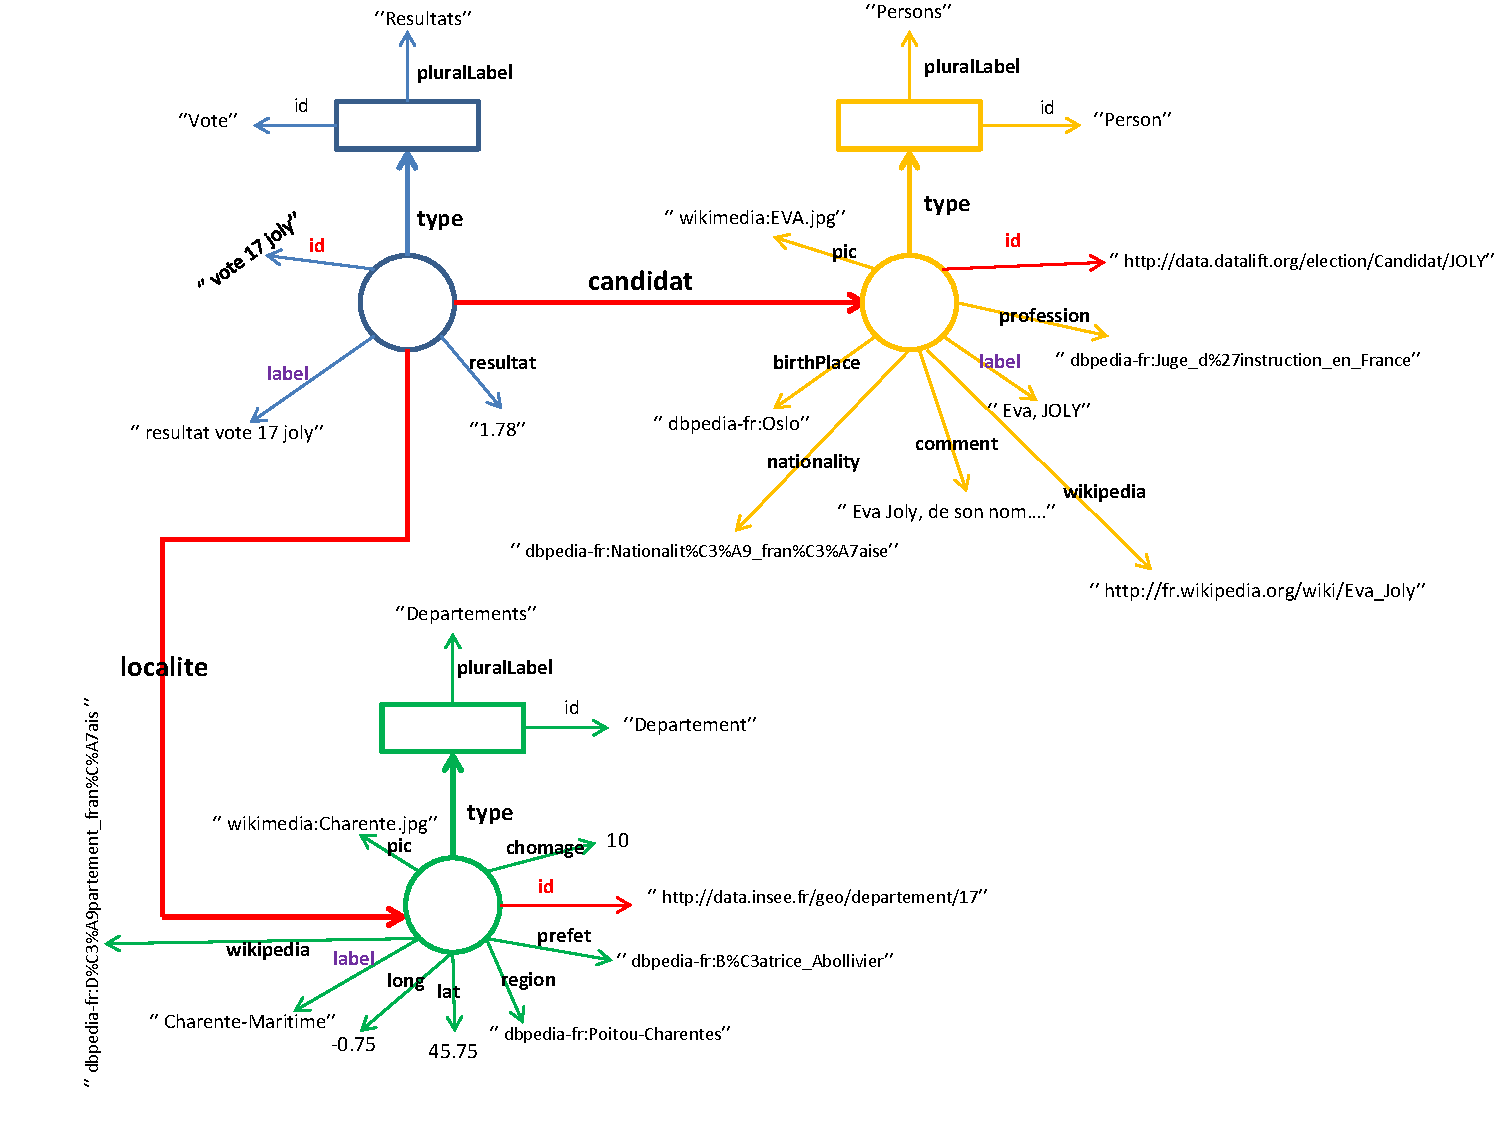
\includegraphics[height=5in]{model_EvaJoly_data}
    \else
      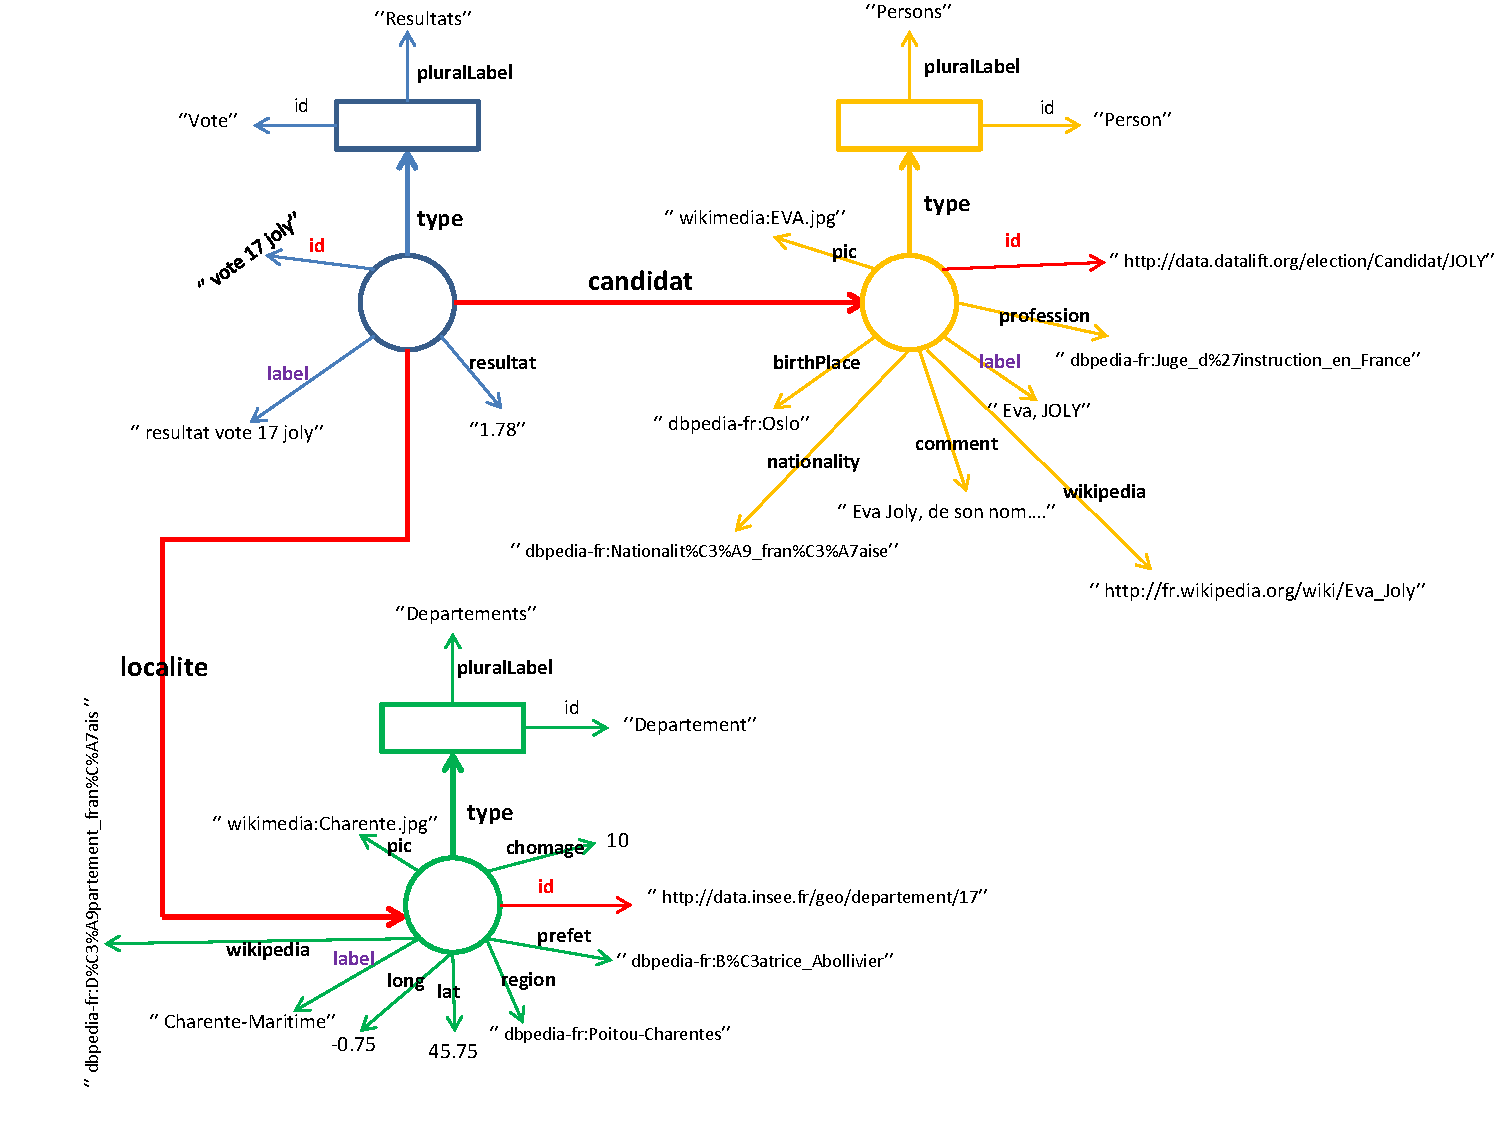
\includegraphics[bb = 92 86 545 742, height=6in]{model_EvaJoly_data}
    \fi
    \caption{Exhibit Data model of the score obtained by candidate Eva Joly in Charente-Maritime, linked with knowledge from DBpedia, INSEE and Wikipedia. }
    \label{sampleModel}
  \end{center}
\end{figure}
\end{landscape}

Regarding tools used for visualization, we have divided them into two categories, providing for each of them relevant examples: (i)-tools that operate over RDF data, (ii) and tools that operate over other structured format. We then provide some basic criteria for assessing a given visualization tool, with some weight attached to each of the criterion. 

 \section{Usage Scenarii for Application}
 
 \section{Tools for Visualizing Data on the Semantic Web}
 
 \section{Towards a Framework For Generating Automatically Visualizations From Linked Data}
  
  \subsection{Requirements}
  \subsection{Specifications}
  \subsection{Implementation}
  
 \section{Linked Open Applications (LOApps)}

%%%%%%%%%%%%%%%%%%%%%%%%%%%%%%%%%%%%
%%%  Conclusions and Future Work %%%
%%%%%%%%%%%%%%%%%%%%%%%%%%%%%%%%%%%%

\chapter*{Conclusions and Future work}
Regarding the geodata modeling, our future work includes the conversion and publication of a large RDF dataset of geographic information of the French territory together with alignments with other datasets at the instance level. At the same time, we plan to publish with IGN a new version of an adequate ontology for describing features and geometry according some best practices we are contributing to elaborate. Furthermore, some alignments with the new OGC standard GeoSPARQL will be performed and evaluated.

Regarding the visualization tools, some further studies should be made for mobile applications, as they are not considered in this current study. We plan also to develop a small vocabulary that could be used to describe OpenData applications. At the same time, we will develop two more applications using different datasets for detecting patterns for visualizing RDF data. For this challenge, we will need to study the underlying data (list of properties, number of triples, categories, etc.), the ontologies used, the templates or libraries for visualizations (Exhibit, GeoAPI, LDA, Sparkl, d3.js,etc) and finally the effort for a user to build the application.


%\cleardoublepage
\addcontentsline{toc}{chapter}{Bibliography}
\nocite{*}
\bibliography{biblio}

%\appendix
%\cleardoublepage
\addcontentsline{toc}{chapter}{Annexes}

\appendix
\chapter{Publications}
\section*{Journal}
\begin{itemize}
\item [1]- Su\'{a}rez-Figueroa, Mari Carmen; Atemezing, Ghislain Auguste; Corcho, Oscar : \textbf{The landscape of 
multimedia ontologies in the last decade} in  Multimedia Tools and Applications, Vol 55, Number 3, December 2011.
\end{itemize}


\section*{Conference}
\begin{itemize}
\item [2]- Atemezing, Ghislain; Troncy, Rapha\"{e}l: \textbf{Comparing vocabularies for representing geographical features and their geometry} in ISWC 2012, 11th International Semantic Web Conference, Terra Cognita, Boston, USA, November 11-15, 2012
\item [3]- Scharffe, Fran\c cois; Atemezing, Ghislain; Troncy, Rapha\"{e}l; Gandon, Fabien; Villata, Serena; Bucher, B\'{e}n\'{e}dicte; Hamdi, Fay\c cal; Bihanic, Laurent; K\'{e}p\'{e}klian, Gabriel; Cotton, Franck; Euzenat, J\'{e}r\^{o}me; Fan, Zhengjie; Vandenbussche, Pierre-Yves; Vatant, Bernard: \textbf{Enabling linked-data publication with the datalift platform} in
AAAI 2012, 26th Conference on Artificial Intelligence, W10:Semantic Cities, July 22-26, 2012, Toronto, Canada.
\item [4]- Atemezing, Ghislain; Troncy, Rapha\"{e}l : \textbf{Vers une meilleure interop\'{e}rabilit\'{e} des donn\'{e}es g\'{e}ographiques fran\c caises sur le Web de donn\'{e}es} in IC 2012, 23\'{e}mes Journ\'{e}es Francophones d'Ing\'{e}nierie des Connaissances, June 25-29, 2012, Paris, France.
\item [5]- Khrouf, Houda; Atemezing, Ghislain; Rizzo, Giuseppe; Troncy, Rapha\"{e}l; Steiner, Thomas:
\textbf{Aggregating social media for enhancing conference experiences} in RAMSS 2012, 1st International Workshop on Real-Time Analysis and Mining of Social Streams, June 4, 2012, Dublin, Ireland.
\item [6]- Khrouf, Houda; Atemezing, Ghislain; Steiner, Thomas; Rizzo, Giuseppe; Troncy, Rapha\"{e}l: 
\textbf{Confomaton: A conference enhancer with social media from the cloud} in ESWC 2012, 9th Extended Semantic Web Conference, May 27-31, 2012, Heraklion, Crete.
\end{itemize}

\section*{Talk}
\begin{itemize}
\item [7]- Bucher, Benedicte; Hart, Glen; Atemezing, Ghislain; Villazon Terrazas, Boris; Bihanic, Laurent; Roensdorf, Carsten; Hamdi, Fay\c cal; Goodwin, John; Troncy, Rapha\"{e}l; Kepeklian, Gabriel; Corcho, Oscar: 
\textbf{A practical introduction to geographical linked data : lift your data} in 
INSPIRE 2012, Infrastructure for Spatial Information in Europe, June 23-27, 2012, Istanbul, Turkey.
\end{itemize}

\section*{W3C Report}
\begin{itemize}
\item [8]- Wood, David; Atemezing, Ghislain; Hyland, Bernadette : 
\textbf{Common Glossary of Terms in Linked Data} W3C Government Linked Data Working Group, 2012.
\end{itemize}


\chapter{Project}
The work reported here has been funded in the ANR Datalift project where we develop technologies for
\begin{itemize}
\item publishing data as RDF graphs: a very simple data format, 
\item linking these data sets together, by identifying equivalent resources in other data sources,
\item describing the vocabulary used in published data through ontologies.
\item developing innovative applications on top of data sets exposed in RDF. 
\end{itemize}

\section*{Meetings}
We have been present in all the different meetings with the rest of the seven partners of the project.
Since our arrival at Eur\'{e}com, we have attended to all the General Meetings planned as follow:
\begin{itemize}
\item 03-04/09/2012, Montpellier (LIRMM)
\item 06-07/06/2012, Grenoble (INRIA-EXMO)
\item 17-18/01/2012, Paris (INSEE)
\item 29-30/09/2011, Sophia Antipolis (INRIA-WIMIX)
\end{itemize}

\section*{Deliverables}
We have produced two deliverables in the context of Datalift project: 
\begin{itemize}
\item \textbf{D6.1 : Usage scenarii for applications (v.1.1)} Authors: \texttt{Ghislain A. Atemezing (EURECOM), Charles Nepote (FING) and Rapha\"{e}l Troncy (EURECOM)}, June, 8th 2012. Reviewed by Fabien Gandon (INRIA) and Thomas Francart (Mondeca). The document describes some innovative applications consuming open data in UK, USA and France. It also shows up some relevant use cases that could be developed in the DataLift platform, considering the type of data  ``lifted'' from the data providers in the project (INSEE, IGN and DILA). It finally captures some requirements from the perspectives of the users.
\item \textbf{D6.2 : Tools for visualizing data on the Semantic Web (v.1.2)} Authors: \texttt{Ghislain A. Atemezing , Rapha\"{e}l Troncy (EURECOM)}, June, 13th 2012. Reviewed by Fabien Gandon (INRIA), Fran\c cois Scharffe (LIRMM) and Franck Cotton (INSEE). The document describes tools that operate over RDF data, revisits those tools that operate over other structured format, and finally provides some criteria to take into account when selecting a given visualization tool, with some weight attached to each of the criterion.
\end{itemize}

\end{document}